\documentclass[answers,10pt]{exam}

\usepackage{graphicx}
\usepackage{listings}
\usepackage{amssymb}
\usepackage{float} %figure inside minipage
\usepackage{amsmath} % for maxing matrices easier

\newcommand{\B}[1]{\boldsymbol{#1}}
\newcommand{\R}{\mathbb{R}}
\newcommand{\changes}[1]{{\color{red} #1}}
\lstset{breaklines = true}
\usepackage{xcolor}
\usepackage[english]{babel}
\usepackage{amsmath,amssymb,amsthm,mathdots}
\usepackage{graphicx}
\usepackage[colorinlistoftodos]{todonotes}


\renewcommand{\thequestion}{\arabic{question} }
\renewcommand\questionlabel{\llap{\thequestion)}}


\usepackage{xcolor}
\definecolor{SolutionColor}{rgb}{0.1,0.3,1}

\unframedsolutions
\shadedsolutions
\definecolor{SolutionColor}{rgb}{0.9,0.9,1}
\renewcommand{\solutiontitle}{\textbf{Solution}$:\>$  }




%Mathcal and 
\newcommand{\mb}[1]{\mathbb{#1}}
\newcommand{\mc}[1]{\mathcal{#1}}

%Various possibilities for norms
\newcommand{\norm}[2]{\|#1\|_{#2}}
\newcommand{\normtwo}[1]{\|#1\|_{2}}
\newcommand{\normp}[1]{\|#1\|_{p}}

\newcommand{\rn}{\mathbb{R}^n}
\newcommand{\rnn}{\mathbb{R}^{n\times n}}
\newcommand{\rmn}{\mathbb{R}^{m\times n}}



%Boldface for vectors and tildes
\renewcommand{\vec}[1]{{#1}•}
\newcommand{\mat}[1]{{#1}•}

\newcommand{\vect}[1]{\widetilde{\boldsymbol{#1}}}
\newcommand{\matt}[1]{\widetilde{\boldsymbol{#1}}}

%Column and row equivalence
\newcommand{\roweq}{\stackrel{\text{row}}{\sim}}
\newcommand{\coleq}{\stackrel{\text{col}}{\sim}}

\newtheorem{definition}{Definition}
\newtheorem{example}{Example}
\newtheorem{fact}{Fact}
\newtheorem{remark}{Remark}


%Vector spaces
\newcommand{\rank}{\text{rank}\,}
\renewcommand{\dim}{\text{dim}\,}
\newcommand{\Span}[1]{\text{Span}\,\{#1\}}
\newcommand{\basis}[1]{\left\{ #1\right\}}


%Matrix environments
\newcommand{\bmat}[1]{\begin{bmatrix}#1\end{bmatrix}}
\newcommand{\pmat}[1]{\begin{pmatrix}#1\end{pmatrix}}
\newenvironment{amatrix}[1]{%
  \left(\begin{array}{@{}*{#1}{c}|c@{}}
}{%
  \end{array}\right)
}


%Trace and determinant
\newcommand{\diag}{\mathsf{diag}\,}
\newcommand{\range}{\mathsf{range}\,}
\newcommand{\trace}{\mathsf{trace}\,}


\usepackage{hyperref}
\title{MA 402: Project 3}
\author{Matthew Murray, Johnathan Rhyne}
\date{Fall 2019}
\setlength{\marginparwidth}{2cm}
\begin{document}
\maketitle
\textbf{Instructions}: 

\begin{itemize}
\item Detailed instructions regarding submission are available on the class website\footnote{\url{https://github.ncsu.edu/asaibab/ma402_fall_2019/blob/master/projects.md}}.
\item The zip file should contain five files project3.pdf, project3.tex, classnotes.sty, swift.mat, and deblur.mat. 

\item More instructions:
\begin{itemize}
\item MATLAB users: use \verb|loadmat| (type \verb|who| to display what variables are in your workspace. 
\item Python users: use \verb|scipy.io.loadmat|. This will return a dictionary with all the necessary variables.
\end{itemize}
\end{itemize}

\vspace{2mm}


\section{Pen-and-paper exercises}
The problems from this section total $20$ points.
\begin{questions}
\question [10] Consider the matrix $\B{A}$ with the SVD
\[ \B{A} = \bmat{ 4 & 0\\ -5 & -3 \\ 2 & 6} = \B{U} \bmat{6 \sqrt{2}   &  0 \\ 0 & 3\sqrt{2}  \\ 0 & 0} \B{V}^\top , \]
where
\[ \B{U}   = \frac13\bmat{ 1  & -2 &  2 \\ -2  & 1 & 2\\  2 & 2 & 1} \qquad \B{V} = \frac{1}{\sqrt{2}} \bmat{1 & -1 \\ 1  & 1}.  \]
\begin{parts}
\part [0] Verify for yourself that it is indeed the SVD of $\B{A}$, and that $\B{U},\B{V}$ are orthogonal. 
\part [1] What is the rank of this matrix? 
\part [2] From the full SVD of $\B{A}$, write down the reduced SVD of $\B{A}$. 
\part [3] Compute the best rank-$1$ approximation of $A$. 
%\part [1] Call this matrix $A_1$. Find $\|A-A_1\|_F $. 
\part [2] Compute the $2$-norm and the Frobenius norms of $\B{A}$.
\part [2] Using the SVD of $\B{A}$, write down the SVD of $\B{A}^\top$ and $\B{A}^\top \B{A}$. 
\end{parts}
\begin{solution}
\begin{parts}
\part  The SVD of $\B{A}$ is valid. 
\part The rank of a matrix is the maximum number of linearly independent columns or rows of the matrix. Because we have the SVD of $\B{A}$, we can find the rank by counting the number on nonzero singular values of $\B{A}$. \\
$$\therefore rank(\B{A}) = 2$$ 
\part In general, the reduced SVD of a Matrix A is... \\
$$\B{A} = \sum_{j = 1}^{r} \sigma_j\B{u}_j\B{v}_{j}^T$$
where $r$ is the rank of $\B{A}$ and $\B{u}_{j}$ and $\B{v}_{j}$ are the left and right singular vectors of $\B{A}$, respectively. \\
Therefore, the reduced SVD of A is... \\
$$\B{A} = \frac13\bmat{ 1  \\-2\\   2}6 \sqrt{2}\frac{1}{\sqrt{2}} \bmat{1  & 1} + \frac13\bmat{ -2  \\1\\   -2}3 \sqrt{2}\frac{1}{\sqrt{2}} \bmat{-1  & 1} $$
\part The best rank-$k$ approximation of $A$ is...\\
$$ \B{A}_k = \sum_{j = 1}^{k} \sigma_j\B{u}_j\B{v}_{j}^T$$
where $k \leq r$. Here set $k=1$.\\
$$\B{A}_1 = \frac13\bmat{ 1  \\-2\\   2}6 \sqrt{2}\frac{1}{\sqrt{2}} \bmat{1  & 1}$$
\part
$$\|\B{A}\|_F = \sqrt{4^{2}+0^{2}+(-5)^{2}+(-3)^{2}+2^{2}+6^{2}} = \sqrt{90}$$
$$\|\B{A}\|_2 = \sigma _{\max }(\B{A}) = 6\sqrt{2}$$
\part The SVD is... \\
$$\B{A} = \B{U}\bmat{\B{\Sigma}\\0}\B{V}^\top$$
where
\[ \bmat{\B{\Sigma}\\0} = \bmat{6 \sqrt{2}   &  0 \\ 0 & 3\sqrt{2}  \\ 0 & 0} \qquad \B{U}   = \frac13\bmat{ 1  & -2 &  2 \\ -2  & 1 & 2\\  2 & 2 & 1} \qquad \B{V} = \frac{1}{\sqrt{2}} \bmat{1 & -1 \\ 1  & 1}.  \]
$$\therefore \B{A}^\top = (\B{V}^\top)^\top\bmat{\B{\Sigma} & 0}\B{U}^\top =\B{V}\bmat{\B{\Sigma} & 0}\B{U}^\top = \B{V}\bmat{6 \sqrt{2}   &  0 & 0 \\ 0 & 3\sqrt{2} & 0}\B{U}^\top $$
$$\therefore \B{A}^\top\B{A} = \B{V}\bmat{\B{\Sigma} & 0}\B{U}^\top\B{U}\bmat{\B{\Sigma}\\0}\B{V}^\top = \B{V}\bmat{\B{\Sigma}^2}\B{V}^\top =\B{V}\bmat{72 &  0 \\ 0 & 18}\B{V}^\top$$

\end{parts}
\end{solution}

\question [10] Let $A \in \rmn. $ Recall: by definition, the Frobenius norm of $\B{A}$ is $\|\B{A}\|_F = \left( \sum_i\sum_j |a_{ij}|^2 \right)^{1/2}$. In this problem, we will derive the formula $$\|\B{A}\|_F=  \left(\sigma_1^2 + \dots + \sigma_r^2 \right)^{1/2}. $$ 
\begin{parts}
\part  The trace of a square matrix is the sum of its diagonals entries. Show (an alternative representation for the Frobenius norm): 
\[ \|\B{A}\|_F = \left( \trace(\B{A}^\top \B{A}) \right)^{1/2}. \]
\part Let $\B{C},\B{D}$ be $n\times n$ square matrices. Show: $\trace(\B{CD})  = \trace(\B{DC})$. \\
{\em Remark}:  This is known as the cyclic property of trace, which is true despite the fact that in general $\B{CD}\neq \B{DC}$. A consequence of the cyclic property is: if $\B{E}$ has the same size as $\B{C,D}$, it implies 
\[ \trace(\B{CDE}) = \trace(\B{DEC}) = \trace(\B{ECD}). \]
\part Using parts (a and b) complete the proof to show  $\|\B{A}\|_F =  \left(\sigma_1^2 + \dots + \sigma_r^2 \right)^{1/2}$.
\part Show: $ \|\B{A}\|_2 \leq \|\B{A}\|_F \leq \sqrt{r} \|\B{A}\|_2$. 
\end{parts}

\begin{solution}
\begin{parts}
%Begins part a
\part We know that, by definition, the $i^{th}$ row of $\B{A}$ is the $i^{th}$ column of $\B{A}^\top$ and that $i^{th}$ column of $\B{A}$ is the $i^{th}$ row of $\B{A}^\top$ \\
\\
Now, we let $a_i$ be the $i^{th}$ row of $\B{A}$ and $a_i^\top$ be the $i^{th}$ column of $\B{A}^\top$ \\
We also know that if $\B{A}$ is an mxn matrix then $\B{A}^\top\B{A}$ is nxn\\

We can write $\B{A}^\top\B{A}$ as $\sum_{i=1}^{n}{a_i^\top a_i}$
\\
\\
If we look at a general $a_i^\top a_i$ we notice the following: 

\[ \bmat{ a_{i 1} \\ a_{i 2}\\ ...\\  a_{i n}} \qquad \bmat{a_{i 1} & a_{i 2} & ... & a_{i n}}  \]
We are allowed to represent this outer product using the same elements since we are looking at $\B{A}^\top\B{A}$ \\ \\
Since we only care about the diagonal of the product, we will only consider the diagonal of each outer product, which will take the form of the following: 

\[ \bmat{a^2_{i 1} &  &  & \\  & a^2_{i 2} &  &  \\ & & ... &  \\ & & & a^2_{i n}} \]
 From the above matrix, we can see that we need to sum up $n$ number of rows of $\B{A}$ and columns of $\B{A}^\top$. \\
 Using this information, we notice that the $j^{th}$ diagonal element of $\B{A}^\top\B{A}$ can be written as: 
 \begin{equation} \label{a1}
     \sum_{i = 1}^{n}{a^2_{ij}}
 \end{equation} 
 
 
 Since $\trace(\B{A}^\top\B{A})$ is the sum of its diagonal elements, we must sum \ref{a1} for every $j$ less than or equal to $n$, we get the following summation: 
 \begin{equation} \label{a2}
     \sum_{i = 1}^{n}\sum_{j = 1}^{n}{a_{ij}^2} = \sum_{i = 1}^{n}\sum_{j = 1}^{n}|a_{ij}|^2 = \|\B{A}\|_F^2
 \end{equation}
 
 From \ref{a2} We know that $\trace(\B{A}^\top\B{A}) = \|\B{A}\|_F^2 \implies \sqrt{\trace(\B{A}^\top\B{A})} = \|\B{A}\|_F$ \\
 %End of part a
 
 \part%Begins part b
 Given two general nxn matrices, $\B{C}$ and $\B{D}$, we can represent $\B{DC}$ as: 
 $\sum_{j = 1}^{n} d_j \hat{c}_j$ \\
 Where $d_j$ is the $j^{th}$ column of $\B{D}$ and $\hat{c}_j$ is the $j^{th}$ row of $\B{C}$ \\ \\
 
 Looking at the $j^{th}$ term of this summation, we get the following:
 
 \[ \bmat{ d_{1 j} \\ d_{2 j}\\ ...\\  d_{n j}} \qquad \bmat{c_{j 1} & c_{j 2} & ... & c_{j n}}  \] And when we multiply this outer product, we get a matrix with the following diagonal elements: 
 
 \[ \bmat{ d_{1 j} c_{j 1} &  &  & \\  & d_{2 j} c_{j 2} &  &  \\ & & ... &  \\ & & & d_{n j} c_{j n}} \]
 
 Which means we can write the $\trace(d_j \hat{c}_j)$ as $\sum_{i = 1}^n d_{ij} c_{ji}$
 
 To find the trace of $\B{DC}$ we need only sum up each diagonal for every j less than or equal to n, or: 
 
 $$
 \trace(\B{DC}) = \sum_{i = 1}^n\sum_{j = 1}^n d_{ij} c_{ji}
 $$ 
 
 By swapping $\B{C} and \B{D}$ we also get the following: 
 
 $$
 \trace(\B{CD}) = \sum_{i = 1}^n\sum_{j = 1}^n c_{ij} d_{ji}
 $$
 We will prove the following equation holds for every $n \in \mathbb{R}$
 \begin{equation}\label{b1}
     \trace(\B{CD}) = \trace(\B{DC})
 \end{equation}
 To show that (\ref{b1}), we prove by induction:
 \begin{proof}
 Show (\ref{b1}) holds for n = 1: \\
 $$
 \trace(\B{CD}) = \sum_{i = 1}^1\sum_{j = 1}^1 c_{ij} d_{ji} = c_{11}d_{11} = d_{11}c_{11} = \sum_{i = 1}^1\sum_{j = 1}^1 d_{ij} c_{ji} = \trace(\B{DC})
 $$
 Now we show that (\ref{b1}) holds for an arbitrary $n + 1$ given that $n$ holds:
 $$
 \sum_{i = 1}^{n + 1}\sum_{j = 1}^{n + 1} c_{ij} d_{ji} = \sum_{i = 1}^{n + 1}\sum_{j = 1}^{n} c_{ij} d_{ji} + \sum_{i = 1}^{n + 1} c_{ij} d_{ji} = \sum_{i = 1}^{n + 1}\sum_{j = 1}^{n} c_{ij} d_{ji} + \sum_{i = 1}^{n} c_{ij} + c_{n + 1 \  n + 1}d_{n + 1 \  n + 1}
 $$
 We must now look at the first term and get: 
 $$
 \sum_{i = 1}^{n + 1}\sum_{j = 1}^{n} c_{ij} d_{ji} = \sum_{i = 1}^{n}\sum_{j = 1}^{n} c_{ij} d_{ji} + \sum_{j = 1}^{n}c_{ij} d_{ji}
 $$
 Combining both the above equations we get the following: 
 
 $$
 \sum_{i = 1}^{n + 1}\sum_{j = 1}^{n + 1} c_{ij} d_{ji} = \sum_{i = 1}^{n}\sum_{j = 1}^{n} c_{ij} d_{ji} + \sum_{j = 1}^{n}c_{ij} d_{ji} + \sum_{i = 1}^{n} c_{ij}d_{ji} + c_{n + 1 \  n + 1}d_{n + 1 \  n + 1}
 $$
 By both our induction hypothesis and the commutativity of numbers in a field (both Real and Complex numbers) we rewrite above as: 
 
 $$
 \sum_{i = 1}^{n}\sum_{j = 1}^{n} d_{ji} c_{ij} + \sum_{j = 1}^{n}d_{ji} c_{ij} + \sum_{i = 1}^{n} d_{ji}c_{ij} + d_{n + 1 \  n + 1}c_{n + 1 \  n + 1}
 $$
 Reversing our methods from above, we get the following: 
 
 $$
 \sum_{i = 1}^{n + 1}\sum_{j = 1}^{n + 1}  d_{ji} c_{ij}
 $$
 
 Since this still cycles through every term of $\B{D} \text{ and } \B{C}$, we can flip the $i$ and $j$ to get: 
 $$
 \sum_{i = 1}^{n + 1}\sum_{j = 1}^{n + 1}  d_{ij} c_{ji} = \trace(\B{DC})
 $$
 
 $\therefore $ we have shown that $\trace(\B{CD}) = \trace(\B{DC})$ for $\B{C},\B{D} \in \mathbb{R}^{nxn}$
 
 \end{proof}
 
 %End of part b
 
 %Starting part c
 
 \part 
 Since $\B{A}^\top\B{A}$ is $nxn$ regardless of if $\B{A}$ has more rows than columns, more columns than rows, or the same number of each, and that we have proved in class that $\B{A}^\top\B{A}$ always takes the form of: 
 
\begin{equation} \label{c1}
     \B{V\Sigma}^2\B{V}^\top
\end{equation}
 We need only to look at (\ref{c1}).\\
 
 As stated from the consequence of part b, we know the following
 $$
 \|\B{A}\|_F^2 = \trace(\B{A}^\top\B{A}) = \trace(\B{V\Sigma}^2\B{V}^\top) = \trace(\B{V}\B{V}^\top\B{\Sigma}^2) = \trace(\B{\Sigma}^2)
 $$
 
 We also know that, by construction, $\sigma_n \geq \sigma_{n + 1}$ and that $\exists r \leq n \ni \sigma_{r + 1} = \dots = \sigma_n = 0$
 \\
 Therefore, we get the following:
 
 $$
 \trace(\Sigma^2) = \sum_{i = 1}^n \sigma^2_i = \sum_{i = 1}^r \sigma^2_i + \sum_{i = r + 1}^n \sigma^2_i = \sum_{i = 1}^r \sigma^2_i + 0 = \sum_{i = 1}^r \sigma^2_i
 $$
 
 $$
 \therefore \|\B{A}\|_F^2 = \trace(\Sigma^2) = \sum_{i = 1}^r \sigma^2_i \implies \|\B{A}\|_F = \sqrt{\sum_{i = 1}^r \sigma^2_i}
 $$
 % Ending of part c
 
 %beginning part d
 \part
 By definition, $\|\B{A}\|_2 = \sigma_1$
 
 $$
 \|\B{A}\|_2 = \sigma_1 = \sqrt{\sigma_1^2} \leq \sqrt{\sigma_1^2 + \dots + \sigma_r^2} = \|\B{A}\|_F \implies \|\B{A}\|_2 \leq \|\B{A}\|_F
 $$
 
 For the second part of the inequality, we must first prove that $r\sigma_1^2 \geq \sum_{i = 1}^r\sigma_i^2$
 
 \begin{proof}
 let r = 1 then we have:
 $$
 \sigma_1^2 \geq \sigma_1^2
 $$
 Which is trivially true
 \\
 Now we look at $r = n \ni n \leq q - 1$ where A is a matrix of size $qxq$
 \\
 $$
 n\sigma_1 \geq \sum_{i = 1}^n\sigma_i^2 \implies n \geq \frac{\sigma_1^2}{\sigma_1^2} + \frac{\sigma_2^2}{\sigma_1^2} + \dots + \frac{\sigma_n^2}{\sigma_1^2} \implies n \geq 1 + \frac{\sigma_2^2}{\sigma_1^2} + \dots + \frac{\sigma_n^2}{\sigma_1^2}
 $$
 By adding 1 to both sides, we get the following:
 $$
 n + 1 \geq 1 + \frac{\sigma_2^2}{\sigma_1^2} + \dots + \frac{\sigma_n^2}{\sigma_1^2} + 1
 $$
 
 We must also note that by construction that $\sigma^2_1 \geq \sigma^2_n \geq \sigma^2_{n + 1}$\\
 Which gives us $1 \geq \dfrac{\sigma^2_n}{\sigma^2_1} \geq  \dfrac{\sigma^2_{n + 1}}{\sigma^2_1} $
 
 Therefore, we can rewrite $n + 1$ as: 
 $$
 n + 1 \geq 1 + \frac{\sigma_2^2}{\sigma_1^2} + \dots + \frac{\sigma_n^2}{\sigma_1^2} + \dfrac{\sigma^2_{n + 1}}{\sigma^2_1} \implies (n + 1)\sigma_1^2 \geq \sum_{i = 1}^{n + 1}\sigma_i^2
 $$
 Therefore we have shown that $r\sigma_1^2 \geq \sum_{i = 1}^r\sigma_i^2$ $\forall r\in\mathbb{N} $ \\\\
 
  We also know that $\sqrt{r\sigma_1^2} \geq \sqrt{\sum_{i = 1}^r\sigma_i^2}$ \\\\
 We have now shown that $\|\B{A}\|_F = \sqrt{\sum_{i = 1}^r\sigma_i^2} \leq \sqrt{r\sigma_1^2} = \sqrt{r}\sqrt{\sigma_1^2} = \sqrt{r}\sigma_1 = \sqrt{r}\|\B{A}\|_2$
 \\\\
 Finally, we have proven that $ \|\B{A}\|_2 \leq \|\B{A}\|_F \leq \sqrt{r} \|\B{A}\|_2$
 
 \end{proof}

 
 \end{parts}

\end{solution}

\section{Numerical exercises}

The problems from this section total $30$ points.  



\question [15] {\em Compressing} and {\em Denoising} images.  
\begin{parts}
\part [0] Load the file `swift.mat'. You will find the variables \verb|A| and \verb|An| which are both matrices  of size $512\times 1024$. 
\part [2] In a single figure with 2 subplots, plot the clean as well as the noisy matrices as images. Denote the corresponding matrices as $\B{A}$ and $\tilde{\B{A}} = \B{A} + \B{E}$, where $\B{E}$ represents the noise that is added to the original image. Unfortunately, in real applications we do not know exactly how much noise is added.  
\part [2] Plot the first $100$ singular values of $\B{A}$ and $\tilde{\B{A}}$. ({\em Hint:} Use the \verb|semilogy| plotting function).  
\part [3] In a single figure with 9 different subplots, plot $\B{A}_k$ (the best rank-$k$ approximation to $\B{A}$) as images for $k = 10,20,\dots,90$ (use these same values of $k$ for the rest of this problem). 
\part  [2] As two subplots of the same figure, plot (left panel) the storage cost of the truncated SVD as a function of $k$, (right panel) relative error of $\B{A}_k$ (in the Frobenius norm) as a function of $k$. Comment on these two subplots. (Assume that each floating point number requires $1$ unit of storage.)
\part [3] Our proposed algorithm to denoise the image is to use a truncated SVD of the matrix corresponding to the noisy image, i.e., computing $\tilde{\B{A}}_k$. In a single figure with 9 different subplots, plot $\tilde{\B{A}}_k$ (the best rank-$k$ approximation to $\B{A}$) as images for $k = 10,20,\dots,90$. Make sure to label each subplot.
\part [2] Plot the relative error of the denoised image $\tilde{\B{A}}_k$ (in the Frobenius norm) as a function of the truncation index $k$. For (approximately) what value of $k$ is the minimum attained?
\end{parts}
{\em Instructions}: In total, you have to submit $6$ separate plots. Make sure to label each plot/subplot, and label the axes of the singular value and the error plots. MATLAB users may want to use commands like \begin{verbatim}figure, image(A), colorbar, colormap(gray(256))\end{verbatim} Python users may want to try \verb|imshow|.
\begin{solution}
\begin{parts}
\part Loaded Swift.m 
\part Clean and Noisy Matrices
\begin{figure}[H]
    \centering
    \text{$\B{A}\text{ and }\tilde{\B{A}}=\B{A}+\B{E}$}\par\medskip
    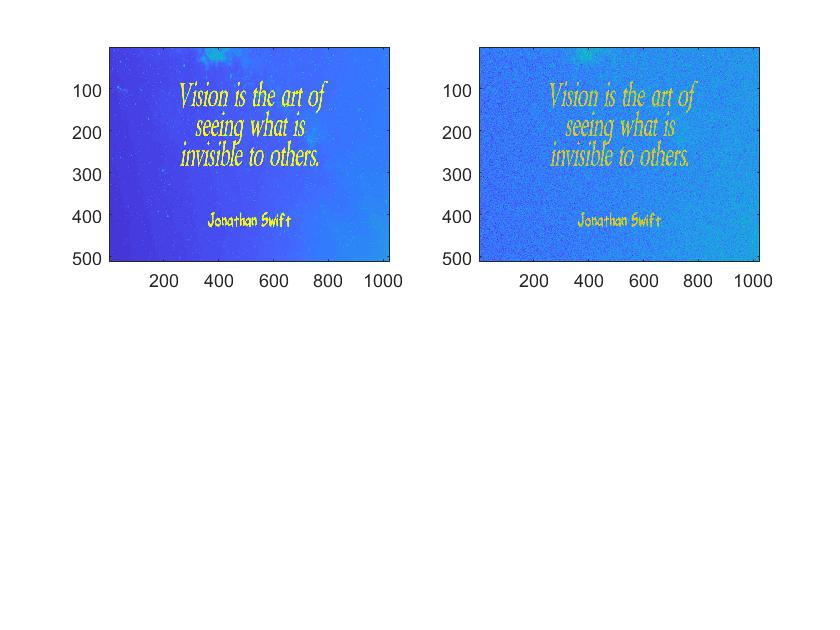
\includegraphics[width=5in]{cleannoisy.jpg} 
    \caption{Image of Clean and Noisy Matrices} 
    \label{fig:my_label1}
\end{figure}
\part First 100 Singular Values
\begin{figure}[H]
    \centering
    \text{\text{First 100 Singular Values of }$\B{A}\text{ and }\tilde{\B{A}}$}\par\medskip
    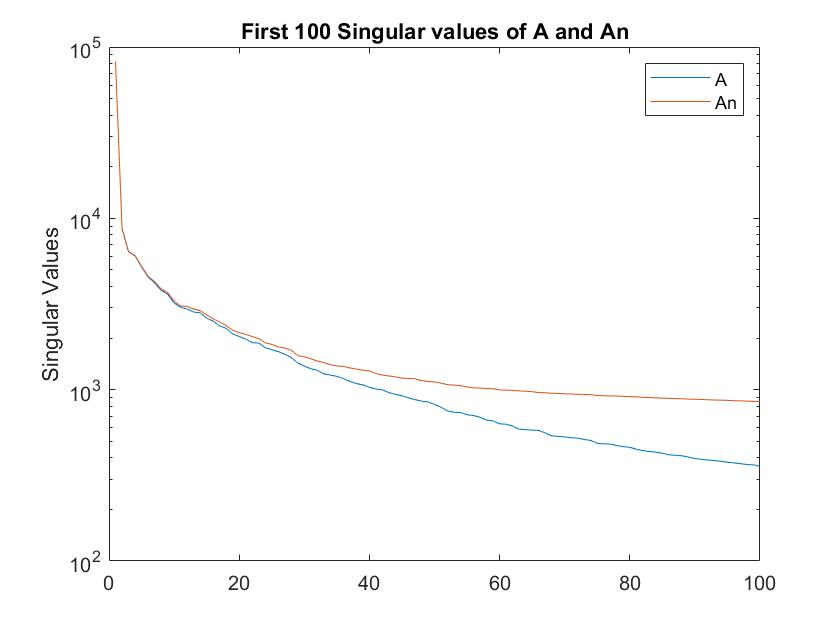
\includegraphics[width=5in]{100SVs.jpg} 
    \caption{Plot of First 100 Singular Values} 
    \label{fig:my_label1}
\end{figure}
\part Best Rank-k Approximation
\begin{figure}[H]
    \centering
    \text{Best Rank-k Approximation, $\B{A}_{k}$, for $k = 10,20,...,80,90$}\par\medskip
    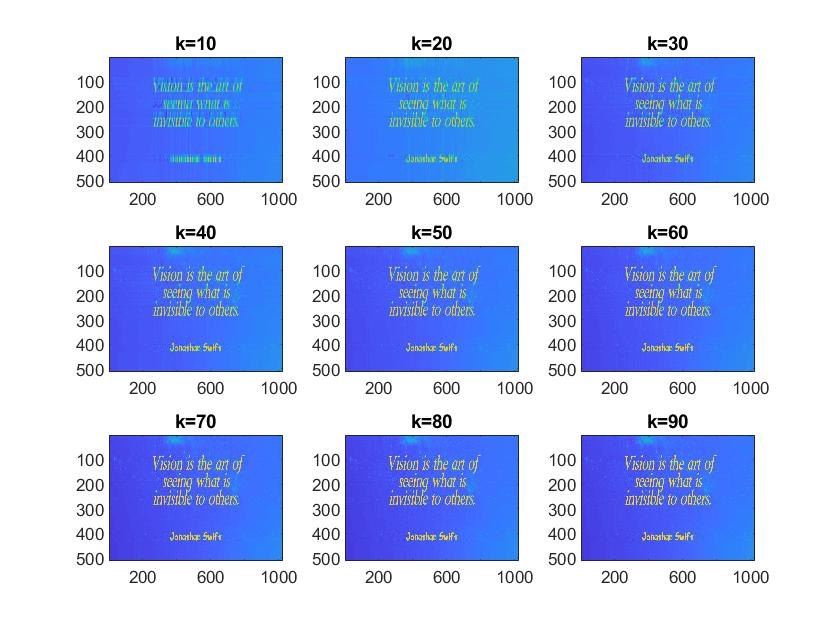
\includegraphics[width=5in]{Akapprox.jpg} 
    \caption{$\B{A}_{k}$, for $k = 10,20,...,80,90$} 
    \label{fig:my_label1}
\end{figure}
\part Storage Cost and Relative Error
\begin{figure}[H]
    \centering
    \text{Storage Cost and Relative Error}\par\medskip
    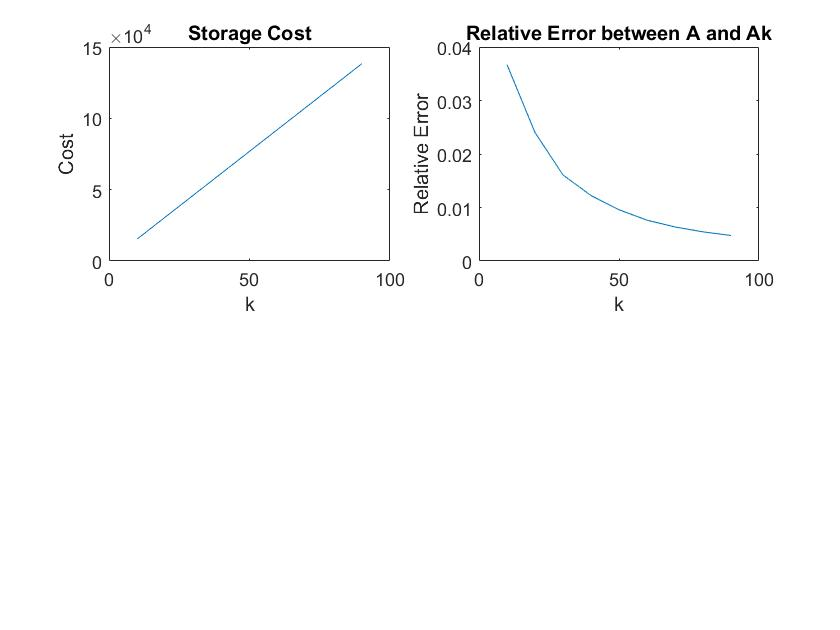
\includegraphics[width=5in]{costrelerror.jpg} 
    \caption{Storage Cost of $\B{A}_{k}$ and Relative Error between $\B{A} \text{ and } \B{A}_k$} 
    \label{fig:my_label1}
\end{figure}
The storage cost is linearly proportional to k. More specifically the cost, $C(k) = (m+n+1)k$. The relative error should improve as more terms are added(the relative error decreases as $k$ increases.)
\part Best Rank-k Approximation
\begin{figure}[H]
    \centering
    \text{Best Rank-k Approximation, $\B{\tilde{A}}_{k}$, for $k = 10,20,...,80,90$}\par\medskip
    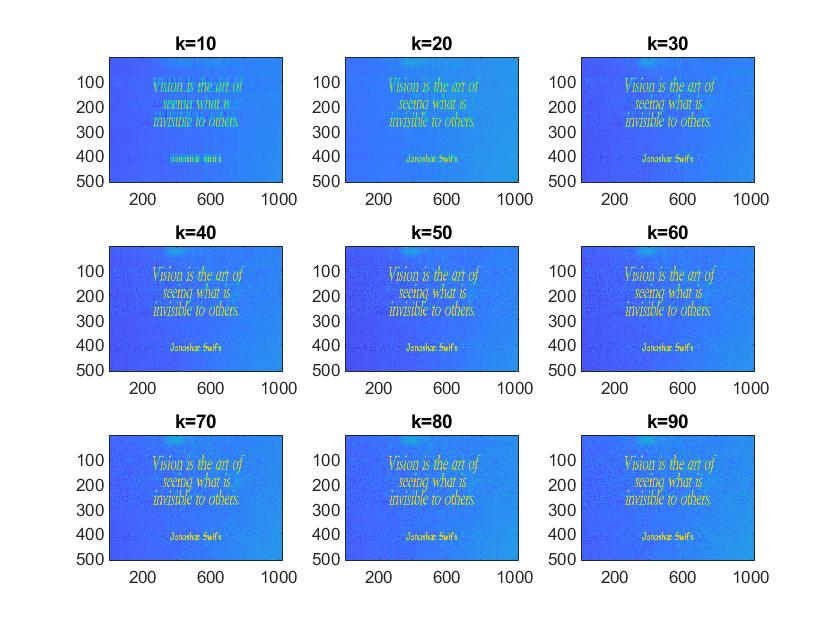
\includegraphics[width=5in]{Ankapprox.jpg} 
    \caption{$\B{\tilde{A}}_{k}$, for $k = 10,20,...,80,90$} 
    \label{fig:my_label1}
\end{figure}
\part Relative Error
\begin{figure}[H]
    \centering
    \text{Relative Error}\par\medskip
    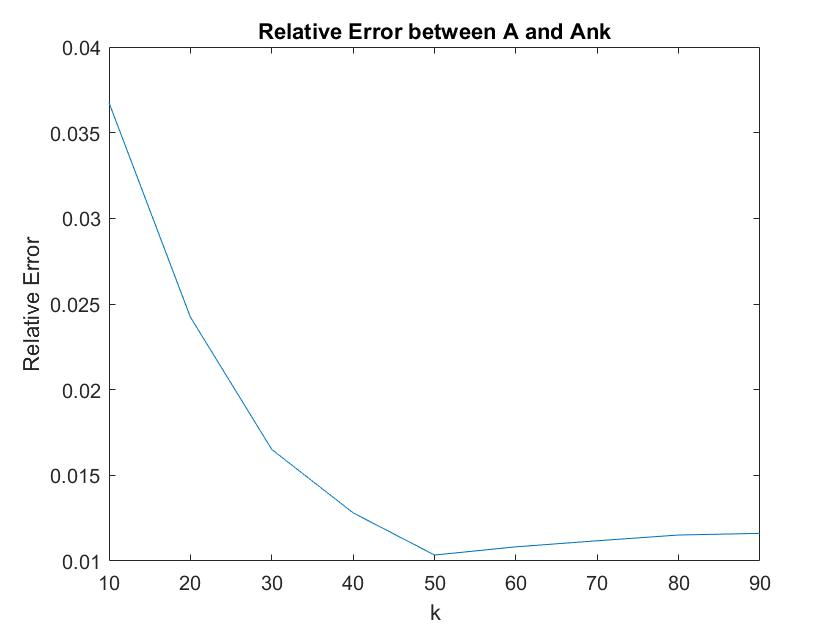
\includegraphics[width=5in]{Anrelerror.jpg} 
    \caption{Relative Error between $\B{A} \text{ and } \B{\tilde{A}}_k$} 
    \label{fig:my_label1}
\end{figure}
The minimum occurs at approximately $k=50$. 
\end{parts}
\end{solution}

\question [15] {\em Deblurring} an image. 
\begin{parts}
\part [0] Load the file `deblur.mat'. You will find the variables \verb|A|  (blurring operator, size $4096\times 4096$) and \verb|bn| (blurred and noisy image, size $4096\times 1$), \verb|xtrue| (true image, size $4096\times 1$). 
\part [2] In a single figure with 2 subplots, plot the true image,  and the blurry image with noise. Note that you will have to reshape the vectors into $64\times 64$ images. 
\part [2] Recall the naive solution $\B{x}_\text{naive} = \B{A}^{-1}{\B{b}_\text{noisy}}$. Plot this solution as an image. (MATLAB users should look up backslash \verb|\|, and Python users should look up \verb|numpy.linalg.solve|. Do not compute the inverse of the matrix!) 
\part [3] Compute the condition number $\kappa_2(\B{A}) = \|\B{A}\|_2 \|\B{A}^{-1}\|_2$ of the matrix $A$. Using perturbation analysis explain why you expect the naive solution to perform poorly (you are given that $\|\B{e}\|_2/\|\B{b}\|_2 = {0.05}$). 
\part [3] Implement the truncated SVD formula 
\[ \B{x}_k = \sum_{j=1}^k \B{v}_j \frac{\B{u}_j^\top {\B{b}_\text{noisy}}}{\sigma_j} , \]
for $k = 400,800,\dots,3600$. In a single figure with 9 subplots, plot the reconstructed vectors $\B{x}_k$ as images. 
\part [3] Plot the relative error in the reconstructed solution as a function of $k$. For (approximately) what value of $k$ is the minimum attained? 
\part [2] In your words, explain the behavior of the error as a function of $k$. 
\end{parts}
{\em Instructions}: In total, you have to submit $4$ separate plots. Make sure to label each plot/subplot, and label the axes of the error plots.
\begin{solution}
\begin{parts}
\part Loaded Deblur.m
\part The True Image and the Blurry, Noisy Image
\begin{figure}[H]
    \centering
    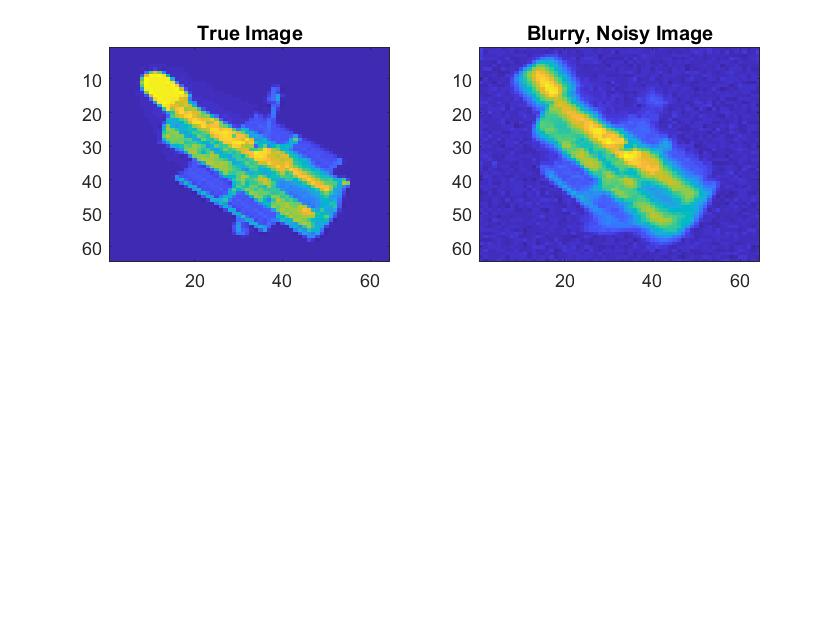
\includegraphics[width=5in]{trueandnoisyblurry.jpg} 
    \caption{The True Image and the Blurry, Noisy Image} 
    \label{fig:my_label1}
\end{figure}
\part The Naive Deblurring Solution
\begin{figure}[H]
    \centering
    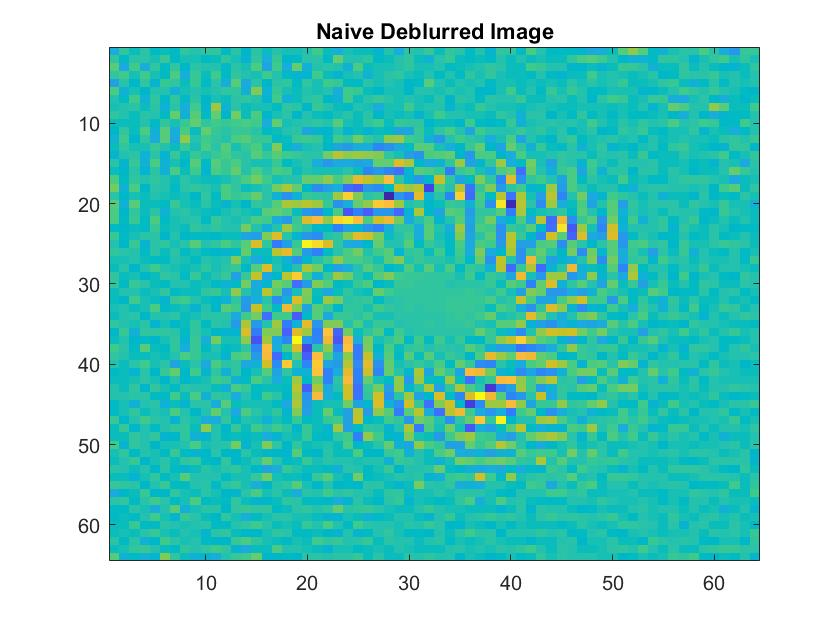
\includegraphics[width=5in]{naivedeblurred.jpg} 
    \caption{The Naive Deblurred Image} 
    \label{fig:my_label1}
\end{figure}
\part The condition number $\kappa_2(\B{A}) = 5.0399*10^{3}$.\\
The naive soultion fails because the noise is being amplified by the condition number. Then, the relative error in the naive solution satisfies:
$$\frac{\|\B{x}_\text{naive} - \B{x}_\text{true}\|_2}{\|\B{x}_\text{true}\|} \leq \|\B{A}\|_2 \|\B{A}^{-1}\|_2\frac{\|\B{e}\|_2}{\|\B{b}\|_2} = \kappa_2(\B{A})\frac{\|\B{e}\|_2}{\|\B{b}\|_2}$$
The condition number is much larger than $1$. The relative error in the output is bounded by $5.0399*10^{3}*0.05 = 251.995$. The relative error in the output is large even for a small relative errror in the input. The blurring matrix is ill-conditioned. 
\part The Truncated SVD
\begin{figure}[H]
    \centering
    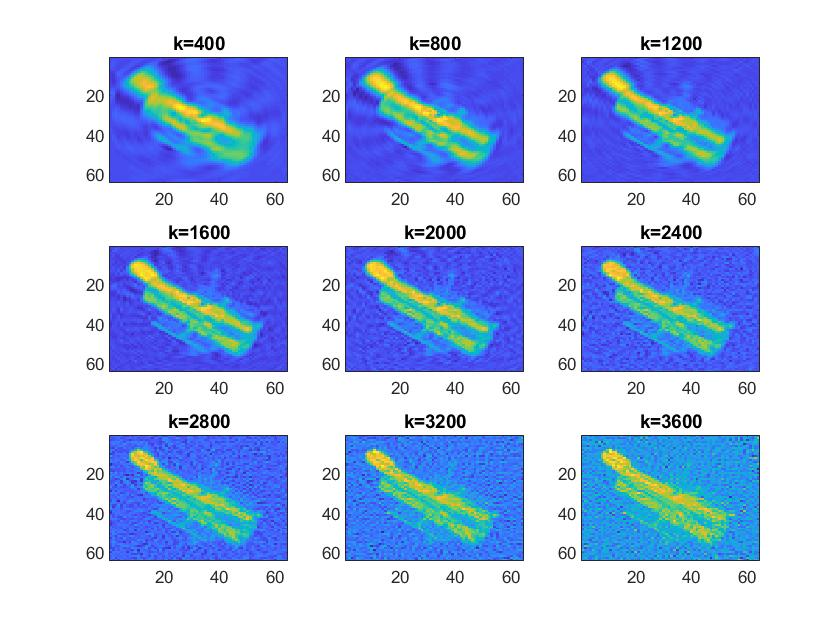
\includegraphics[width=5in]{truncatedsvddeblur.jpg} 
    \caption{Truncated SVD} 
    \label{fig:my_label1}
\end{figure}
The minimum occurs at approximately $k=1600$. 
\part 
\begin{figure}[H]
    \centering
    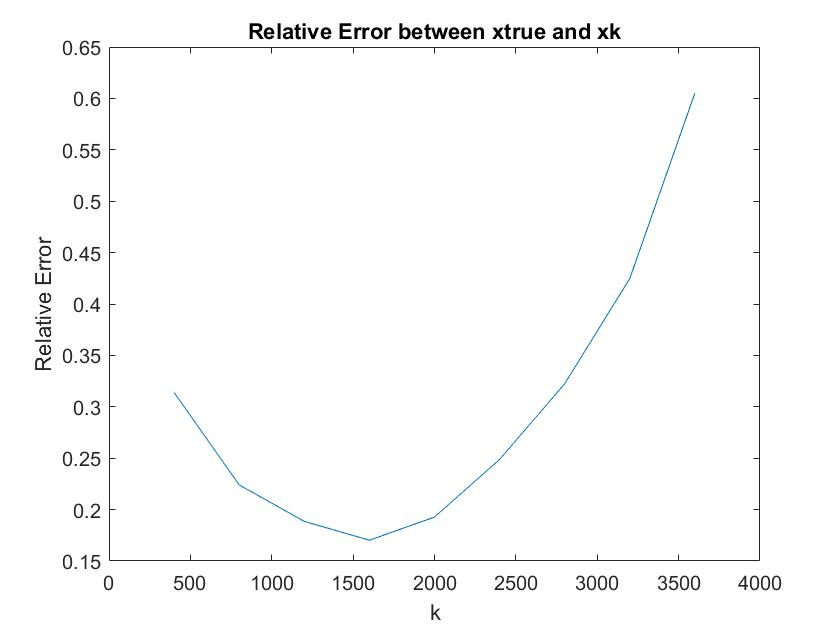
\includegraphics[width=5in]{xtruerelerror.jpg} 
    \caption{Truncated SVD} 
    \label{fig:my_label1}
\end{figure}
The relative error is high for small values of k, reaches a minimum, and then becomes large again for large values of k. The noise becomes more apparent for small k values. For large k values, the terms of the truncated SVD are less important. Therefore, the images are less accurate.  
\end{parts}
\end{solution}


\begin{solution}
$$ $$
For Figure 1
\begin{lstlisting}[language = Matlab]
%Clean and Noisy Images
subplot(2,2,1)
imagesc(A)
subplot(2,2,2)
imagesc(An)
\end{lstlisting}
$$ $$
For Figure 2
\begin{lstlisting}[language = Matlab]
sigma = svd(A); %singular values of A
sigman = svd(An); %singular values of An
semilogy(sigma(1:100))
title('First 100 Singular values of A and An') 
ylabel('Singular Values') 
hold on
semilogy(sigman(1:100))
legend('A','An')
hold off
\end{lstlisting}
$$ $$
For Figure 3
\begin{lstlisting}[language = Matlab]
[U,S,V] = svd(A); %such that A = USV
sigma = svd(A);
k=10:10:90;
 A_k = zeros(512,1024);
 V1 = transpose(V); 
 Title = {'k=10','k=20','k=30','k=40','k=50','k=60','k=70','k=80','k=90'};
 for i=1:9
     for j = 1:k(i)
         A_j = sigma(j)*U(:,j)*V1(j,:); %terms of the truncated SVD
         A_k = A_k + A_j;
     end
 subplot(3,3,i)
 imagesc(A_k)
 title(Title(i))
 A_clean = zeros(512,1024);
 end
\end{lstlisting}
$$ $$
For Figure 4
\begin{lstlisting}[language = Matlab]
sigma = svd(A);
k=10:10:90;
A_k = zeros(512,1024);
V1 = transpose(V);
rel = zeros(9,1);
for i=1:9
    for j = 1:k(i)
        A_j = sigma(j)*U(:,j)*V1(j,:);
        A_k = A_k + A_j;
    end
    rel(i) = norm(A-A_k,2)/norm(A,2); %the relative error using the frobenius norm
    A_k = zeros(512,1024);
end
subplot(2,2,1)
plot(k,cost(k))
title('Storage Cost')
xlabel('k')
ylabel('Cost')
subplot(2,2,2)
plot(k,rel)
title('Relative Error between A and Ak')
xlabel('k')
ylabel('Relative Error')
f = @cost;
function y = cost(x)
m=512;
n=1024;
    y = (m+n+1)*x; %the cost function is linearly proportional to k
end
\end{lstlisting}
$$ $$
For Figure 5
\begin{lstlisting}[language = Matlab]
k=10:10:90;
 An_k = zeros(512,1024);
 Vn1 = transpose(Vn);
 Title = {'k=10','k=20','k=30','k=40','k=50','k=60','k=70','k=80','k=90'};
 for i=1:9
     for j = 1:k(i)
         A_j = sigman(j)*Un(:,j)*Vn1(j,:);
         An_k = An_k + A_j;
     end
 subplot(3,3,i)
 imagesc(An_k)
 title(Title(i))
 An_k = zeros(512,1024);
 end
\end{lstlisting}
$$ $$
For Figure 6
\begin{lstlisting}[language = Matlab]
An_k = zeros(512,1024);
Vn1 = transpose(Vn);
reln = zeros(9,1);
for i=1:9
    for j = 1:k(i)
        An_j = sigman(j)*Un(:,j)*Vn1(j,:);
        An_k = An_k + An_j;
    end
    Q=A-An_k;
    reln(i) = norm(Q,2)/norm(A,2); %the relative error using the frobenius norm
    An_k = zeros(512,1024);
end
plot(k,reln)
title('Relative Error between A and Ank')
xlabel('k')
ylabel('Relative Error')
\end{lstlisting}
$$ $$
For Figure 7
\begin{lstlisting}[language = Matlab]
%Clean Image and Blurry,Noisy Image
Itrue = reshape(xtrue,64,64);
Ibn = reshape(bn,64,64);
subplot(2,2,1)
imagesc(Itrue)
title('True Image')
subplot(2,2,2)
imagesc(Ibn)
title('Blurry, Noisy Image')
\end{lstlisting}


\end{solution}

\end{questions}

\end{document}


